\section{Exploratory analysis and problem framing}
\label{sec:eda}

\subsection{Data integrity}

The raw table has 48{,}842 rows and 14 features: 6 integers and 8 categories. We
checked the meaning of each column, not only its storage type, which led to
three cleaning decisions.
\begin{itemize}
  \item \textbf{Missing values} appear only in three categorical columns:
  \code{workclass} (5.7\%), \code{occupation} (5.8\%) and \code{native-country}
  (1.8\%). They are imputed inside the Pipeline (Section~\ref{sec:features}),
  never before the split.
  \item \textbf{52 exact duplicate rows} (0.1\%) are dropped before the split,
  so the same record cannot end up both in a training fold and in the matching
  validation fold, or both in the development and the test set.
  \item \textbf{Two columns are not given to the model.} \code{education} and
  \code{education-num} have 16 values each and map one-to-one: each label has
  exactly one number and each number exactly one label. We keep
  \code{education-num}, which also carries the order of the levels.
  \code{fnlwgt} is a sampling weight of the census survey: it describes how the
  survey was designed, not the person whose income we predict.
\end{itemize}

\subsection{Validation protocol}

Each row is one person and there is no time dimension, so a random split is
appropriate. We split the cleaned data (48{,}790 rows) once, stratified on the
target, into a development set of 39{,}032 rows and a test set of 9{,}758 rows.
Both contain 23.9\% of \pos. Inside the development set, every comparison uses
the same 5-fold \code{StratifiedKFold} (shuffled, seed 42), so all models are
scored on exactly the same folds. Everything that relates the features to the
target, including the analysis below, was done on the development set only:
looking at the test set would already be a modelling decision.

\subsection{Target and choice of metrics}

The development set has 29{,}687 people at \negc{} and 9{,}345 at \pos. A model
that always predicts \negc{} is already 76.1\% accurate, so accuracy alone says
little. We report the same metrics for every model: ROC-AUC and Average
Precision (AP, the area under the precision-recall curve), which judge how well
people are ranked, without a threshold; log-loss, which judges the
probabilities; and precision, recall, F1 and the confusion matrix, which judge
the final decisions at a given threshold. AP is our selection metric: it focuses
on how well the minority class is retrieved, and its reference value is the
prevalence (0.239), against 0.5 for ROC-AUC.

\subsection{Main findings}

Table~\ref{tab:eda-means} compares the numerical features between the two
classes (the full distributions are in Figure~\ref{fig:eda-numeric}, in the
appendix). People earning \pos{} are older, more educated and work more hours.
\code{capital-gain} and \code{capital-loss} are zero for 91.8\% and 95.2\% of
people, with a long tail of large values. The share of \pos{} rises with age,
peaks around 50 and then falls (Figure~\ref{fig:eda-age}): a curve that a
linear model cannot draw with \code{age} alone. Among the categorical features
(Figure~\ref{fig:eda-categorical}), the household variables separate the
classes most: the share of \pos{} ranges from 5\% to 45\% across
\code{marital-status} values and from 2\% to 47\% across \code{relationship}
values. It is 30\% for men and 11\% for women.

\begin{table}[H]
\centering
\caption{Mean of each numerical feature by class (development set).}
\label{tab:eda-means}
\begin{tabular}{lrrrrr}
\toprule
Class & age & education-num & capital-gain & capital-loss & hours-per-week \\
\midrule
\negc & 36.9 & 9.6 & 144 & 54 & 38.8 \\
\pos  & 44.3 & 11.6 & 4{,}096 & 200 & 45.5 \\
\bottomrule
\end{tabular}
\end{table}

\begin{figure}[H]
\centering
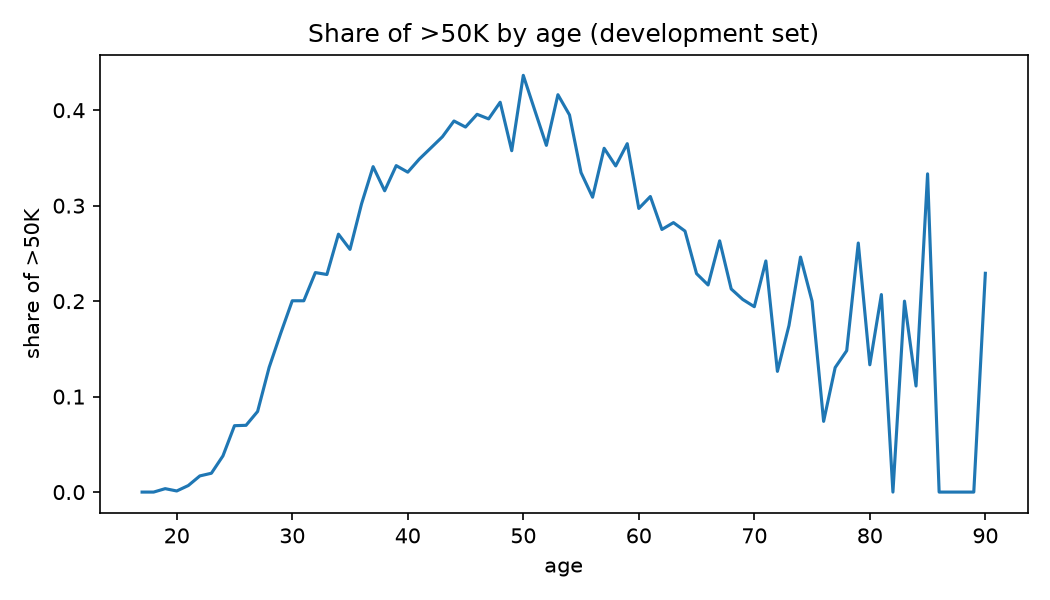
\includegraphics[width=0.55\textwidth]{eda_rate_by_age.png}
\caption{Share of \pos{} by age (development set): an inverted U, which
motivates the \code{age\_squared} feature.}
\label{fig:eda-age}
\end{figure}

\subsection{Leakage audit}

For each feature, we asked whether its value would really be known at the
moment the prediction is made (Table~\ref{tab:leakage}). Personal
characteristics, education, job and household are known in advance.
\code{capital-gain} and \code{capital-loss} are a medium risk: they are declared
for the same tax year as the income, so in production they might only become
available together with the income itself. We keep them, because the census
collects them at the same time as the other answers, but this must be checked
before any real deployment.

\begin{table}[H]
\centering
\caption{Leakage audit: could we know this value when the prediction is made?}
\label{tab:leakage}
\small
\begin{tabular}{p{4.6cm}p{2.4cm}p{2.2cm}p{5.2cm}}
\toprule
Features & Known at prediction time & Risk & Why \\
\midrule
age, sex, race, native-country & Yes & Low & Fixed personal characteristics \\
education-num & Yes & Low & Obtained before the income is earned \\
workclass, occupation, hours-per-week & Yes & Low & Describe the current job \\
marital-status, relationship & Yes & Low & Household situation \\
capital-gain, capital-loss & Same tax year & Medium & Declared with the income \\
fnlwgt & Yes & Not a person feature & Survey weight, dropped \\
\bottomrule
\end{tabular}
\end{table}

\subsection{Open questions}

Two assumptions remain open after the analysis. First, missing \code{workclass}
and \code{occupation} values may not be random: they could describe people who
do not work (we test this in Section~\ref{sec:discussion}). Second, the data
dates from 1994: income levels have changed since, so the \$50K threshold does
not mean the same today, and the model should not be used on recent data
without retraining.
